\documentclass[12pt]{article}
\usepackage{amssymb, amsmath}
\usepackage{fancyhdr,lastpage}
\usepackage{amsmath,amsfonts,amssymb}
\usepackage{graphicx}
\usepackage{stix}
\usepackage{enumitem}
\usepackage{listings}
\tolerance 10000
\headheight 0in
\headsep 0in
\evensidemargin 0in
\oddsidemargin \evensidemargin
\textwidth 6.5in
\topmargin .25in
\textheight 8.7in

\newcommand{\CC}{{\mathbb C}}
\newcommand{\QQ}{{\mathbb Q}}
\newcommand{\RR}{{\mathbb R}}
\newcommand{\ZZ}{{\mathbb Z}}
\newcommand{\NN}{{\mathbb N}}
\newcommand{\FF}{{\mathbb F}}


\newcommand{\Zerobold}{{\boldsymbol 0}}
\newcommand{\Onebold}{{\boldsymbol 1}}
\newcommand{\xbold}{{\boldsymbol x}}

\newcommand{\mfrak}{{\mathfrak m}}

\newcommand{\Acal}{{\mathcal A}}
\newcommand{\Ncal}{{\mathcal N}}
\newcommand{\Pcal}{{\mathcal P}}
\newcommand{\Qcal}{{\mathcal Q}}

\newcommand{\sqbinom}[2]{\genfrac{[}{]}{0pt}{}{#1}{#2}}
\newcommand{\angbinom}[2]{\genfrac{\langle}{\rangle}{0pt}{}{#1}{#2}}

\newcommand{\qddx}{(d/dx)_{q}}

%\newcommand{\pfcl}{\emph{Proof of claim}}
\newenvironment{proof}{\paragraph{Proof: }}{\hfill$\blacksquare$}



\def\multiset#1#2{\ensuremath{\left(\kern-.3em\left(\genfrac{}{}{0pt}{}{#1}{#2}\right)\kern-.3em\right)}}


\DeclareMathOperator{\des}{des}
\DeclareMathOperator{\maj}{maj}
\DeclareMathOperator{\ev}{ev}
\DeclareMathOperator{\Hom}{Hom}
\DeclareMathOperator{\trace}{tr}
\DeclareMathOperator{\inv}{inv}

\newtheorem{problem}{Problem}%[section]

\begin{document}

\begin{center}
{\bf Julio Soldevilla}
\\
{\bf EECS 545 Winter 2018 --- Problem Set 3 }
\end{center}

\begin{problem}
\normalfont
Problem 1
\end{problem}

\begin{proof}

\begin{enumerate}

\item This is problem 1.a where we are using the linear kernel. In figure 1 we show the linear kernel with parameter $C = 1$ and in this case we have $12$ support vectors and figure 1 shows the separating hyperplane. 
\begin{figure}[!htbp]
\centering
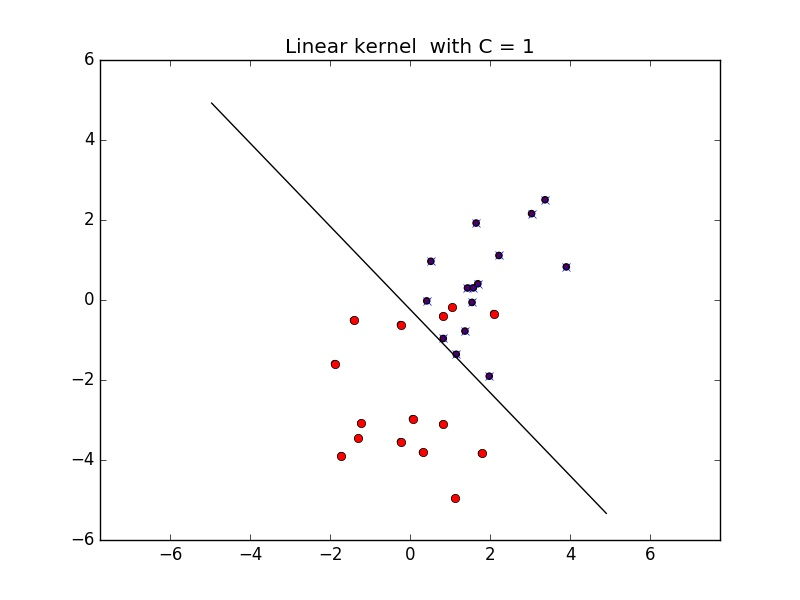
\includegraphics[width=10cm]{prob1_1_linear_C1.jpg}
\caption{\textbf{Problem 1 part a:} Image showing the linear kernel with parameter $C = 1$}
\end{figure} 

After this, we run the linear kernel this time with parameter $C = 100$ and in this case we have $10$ support vectors and figure 2 shows the decision boundary from the algorithm. 

\begin{figure}[!htbp]
\centering
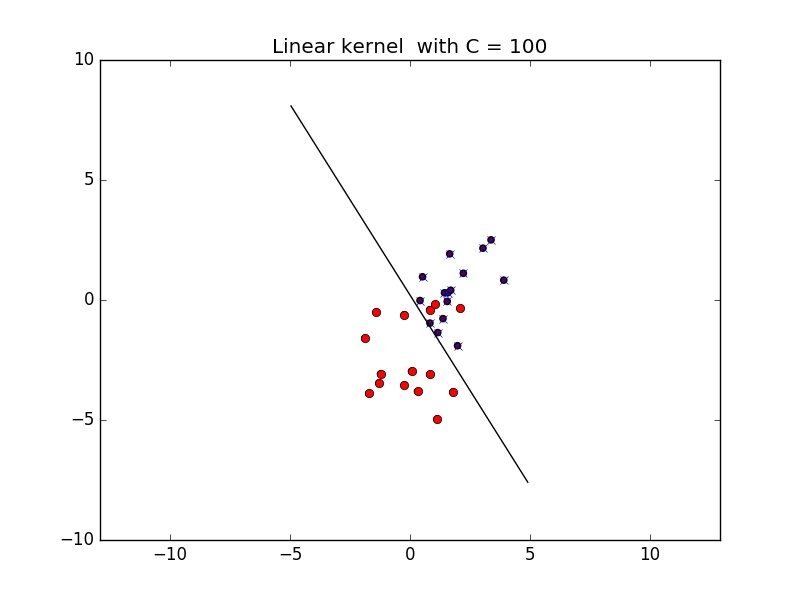
\includegraphics[width=10cm]{prob1_1_linear_C100.jpg}
\caption{\textbf{Problem 1 part a:} Image showing the linear kernel with parameter $C = 100$}
\end{figure} 

\item This is problem 1.b where we are using the rbf kerne. In figure 3 we show the rbf kernel with parameter $C = 1$ and in this case we have $24$ support vectors. Figure 3 shows the decision boundary in this case.

\begin{figure}[!htbp]
\centering
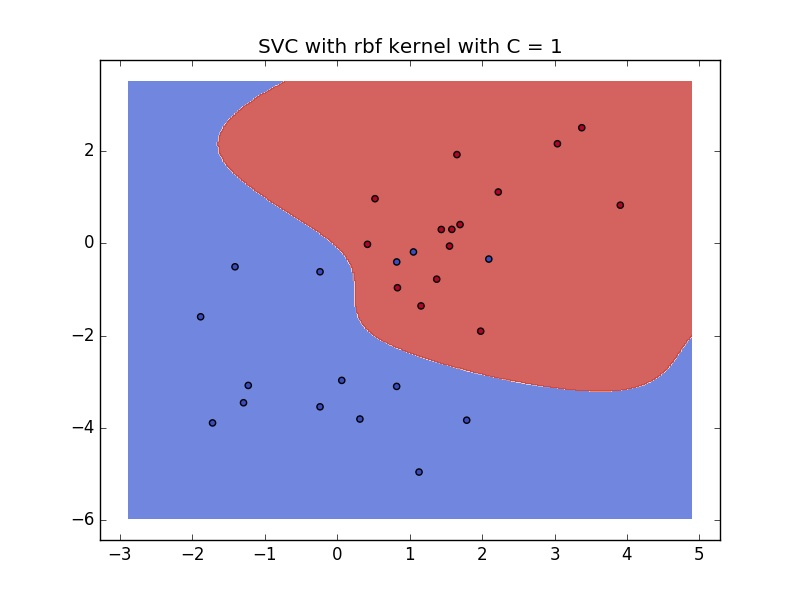
\includegraphics[width=10cm]{prob1_2_rbf_C1.jpg}
\caption{\textbf{Problem 1 part b:} Image showing the rbf kernel with parameter $C = 1$}
\end{figure} 

After this, in figure 4 we show the rbf kernel with parameter $C = 3$ and in this case we have $21$ support vectors. Figure 4 shows the decision boundary in this case.

\begin{figure}[!htbp]
\centering
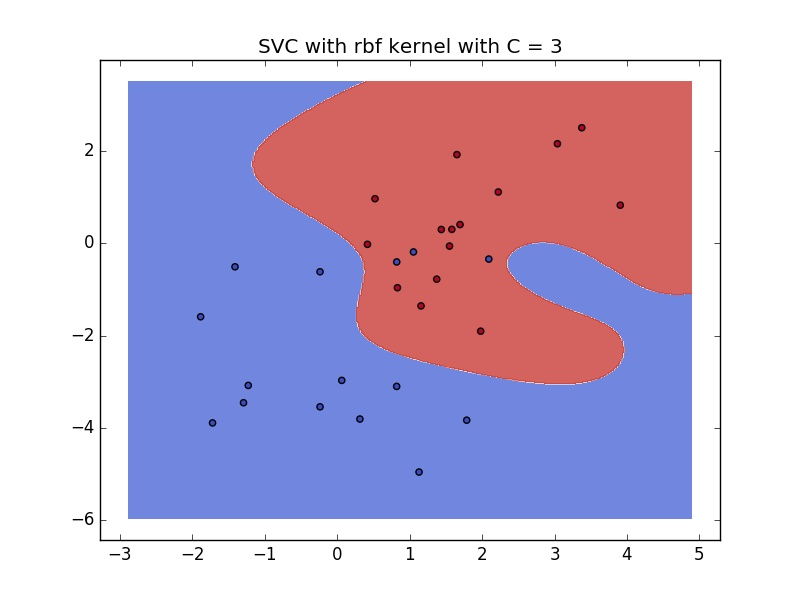
\includegraphics[width=10cm]{prob1_2_rbf_C3.jpg}
\caption{\textbf{Problem 1 part b:} Image showing the rbf kernel with parameter $C = 3$}
\end{figure} 

\end{enumerate}

\end{proof}

\begin{problem}
\normalfont
Problem 2
\end{problem}

\begin{proof}

\begin{enumerate}

\item 

\end{enumerate}

\end{proof}

\end{document}